\documentclass[tikz,border=12pt]{standalone}
\usepackage{amsmath}
\usetikzlibrary{arrows.meta}

\begin{document}
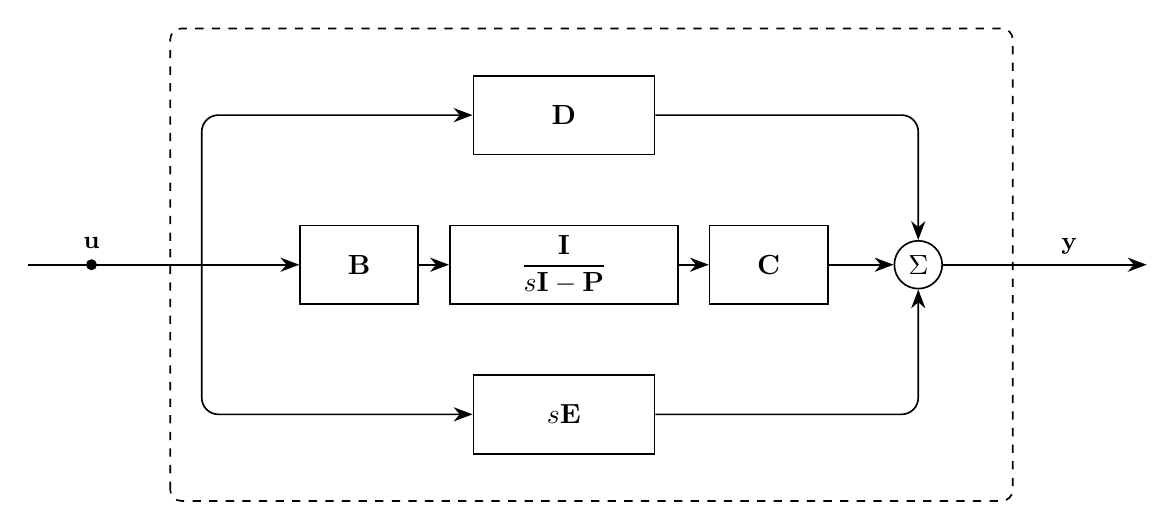
\begin{tikzpicture}[
    >={Stealth[length=2.4mm]},
    line/.style   = {semithick, rounded corners=6pt},
    block/.style  = {draw, semithick, fill=white,
                     minimum height=1cm, minimum width=2.3cm},
    sum/.style    = {draw, semithick, fill=white, circle, inner sep=2.6pt},
    signal/.style = {circle, fill, inner sep=1.4pt, label distance=3pt},
    sig/.style    = {font=\small}
]

% Feedthrough paths
\node[block] (D)  at (0,  1.9) {$\mathbf{D}$};
\node[block] (E)  at (0, -1.9) {$s\mathbf{E}$};

% State-space chain: input map -> resolvent state bank -> output map
\node[block, minimum width=1.5cm] (BT)  at (-2.6, 0) {$\mathbf{B}$};
\node[block, minimum width=2.9cm] (res) at ( 0.0, 0) {$\dfrac{\mathbf{I}}{s\mathbf{I} - \mathbf{P}}$};
\node[block, minimum width=1.5cm] (C)   at ( 2.6, 0) {$\mathbf{C}$};

% Fan-out from a single internal point
\coordinate (split) at (-4.6, 0);
\draw[line] (-6.8, 0) -- (split);
\draw[->, line] (split) -- (BT.west);
\draw[->, line] (split) |- (D.west);
\draw[->, line] (split) |- (E.west);

% Chain series connections
\draw[->, line] (BT.east)  -- (res.west);
\draw[->, line] (res.east) -- (C.west);

% Fan-in to summation
\node[sum] (S) at (4.5, 0) {$\Sigma$};
\draw[->, line] (C.east) -- (S);
\draw[->, line] (D.east) -| (S.north);
\draw[->, line] (E.east) -| (S.south);
\draw[->, line] (S.east) -- (7.4, 0) node[sig, pos=0.62, above] {$\mathbf{y}$};

% Signal node: u external
\node[signal, label={[sig]above:$\mathbf{u}$}] at (-6.0, 0) {};

% Model enclosure
\draw[dashed, semithick, rounded corners=4pt] (-5.0, -3.0) rectangle (5.7, 3.0);

\end{tikzpicture}
\end{document}
